\documentclass[12pt]{article}
\usepackage[margin=0.8in]{geometry}
\usepackage[utf8]{inputenc}
\usepackage{graphicx}
\usepackage[export]{adjustbox}
\usepackage{amsmath}
\usepackage{amsfonts}
\usepackage{amssymb}
\usepackage[version=4]{mhchem}
\usepackage{stmaryrd}
\usepackage{bbold}
%\usepackage[fallback]{xeCJK}
\usepackage{polyglossia}
\usepackage{fontspec}
\usepackage{censor}
%\setCJKmainfont{Noto Serif CJK TC}
\graphicspath{ {../Images/} }
\usepackage{enumitem}
\usepackage{tikz}
\usepackage{amsthm}
\usepackage{tcolorbox}
\usepackage{array}
\usepackage{tabularray}
\usepackage{makecell}
\usepackage{esvect}
%\usepackage{changepage}   % for the adjustwidth environment
\usepackage{enumitem}
\usepackage{tasks}

\tcbuselibrary{theorems}

\definecolor{GrayCen}{HTML}{d2d2d2}
\definecolor{GrayBG}{HTML}{d9d9d9}
\definecolor{BlueDef}{HTML}{104e8b}
\definecolor{GreenProp}{HTML}{025540}
\definecolor{RedMet}{HTML}{cd5556}
\definecolor{BlackSav}{HTML}{000000}
\def\censorcolor{GrayCen}
\let\svcensorrule\censorrule
\renewcommand\censorrule[1]{%
\textcolor{\censorcolor}{\svcensorrule{#1}}}

\newtcbtheorem
[]% init options
{definition}% name
{Définition}% title
{%
  colback=GrayBG,
  colframe=BlueDef,
  fonttitle=\bfseries,
}% options
{def}% prefix

\newtcbtheorem
[]% init options
{proposition}% name
{Proposition}% title
{%
  colback=GrayBG,
  colframe=GreenProp,
  fonttitle=\bfseries,
}% options
{prop}% prefix

\newtcbtheorem
[]% init options
{method}% name
{Méthode}% title
{%
  theorem name,
  colback=GrayBG,
  colframe=RedMet,
  fonttitle=\bfseries,
}% options
{met}% prefix

\newtcbtheorem
[]% init options
{savoir}% name
{Savoir-faire du chapitre}% title
{%
  theorem name,
  colback=GrayBG,
  colframe=BlackSav,
  fonttitle=\bfseries,
}% options
{sav}% prefix

\newtheoremstyle{break}
{\topsep}{\topsep}%
{}{}%
{\bfseries}{}%
{\newline}{}%
\theoremstyle{break}
\newtheorem*{example}{Exemple.}
\newtheorem*{remark}{Remarque.}

\newenvironment{demo}[1][\proofname]{%
  \begin{proof}[#1]$ $\newline
  }{%
  \end{proof}
}

\setmainlanguage{french}
%\setmainfont{CMU Serif}

\title{
  \vspace{4em}
  \centering
  \tcbset{colframe=BlackSav,colback=GrayBG}
  \tcbox[tikznode]{
    Chapitre 9 \\Fonction exponentielle
  }
}

\author{}
\date{}

\setlength\parindent{0pt}
%\setlist[itemize]{topsep=0pt}
\setlist{nolistsep}
%\setlist[itemize]{noitemsep}
%\setlist[enumerate]{noitemsep}

\newcolumntype{C}[1]{>{\centering\arraybackslash}m{#1}}
\newcolumntype{L}[1]{>{\raggedright\arraybackslash}m{#1}}
\newcolumntype{N}{@{}m{0pt}@{}}

\begin{document}
\maketitle

\tableofcontents

\newcommand{\hideM}[1]{\mbox{\vphantom{$#1$}\smash{\colorbox{gray!50}{$\displaystyle #1$}}} }
\newcommand{\hide}[1]{\mbox{\vphantom{#1}\smash{\colorbox{gray!50}{#1}}}}
% \newcommand{\hideM}[1]{\mbox{\vphantom{$#1$}\smash{\colorbox{gray!50}{\phantom{$\displaystyle #1$}}}} }
% \newcommand{\hide}[1]{\mbox{\vphantom{#1}\smash{\colorbox{gray!50}{\phantom{#1}}}}}

\newpage
\section{Définition de la fonction exponentielle et première propriété}
\begin{proposition}{(admise)}{}
  Il existe une unique fonction $f$ définie et dérivable sur $\mathbb{R}$ telle que pour tout $x \in \mathbb{R}$, $f^{\prime}(x)=\hideM{f(x)}$ et telle que $f(0)=1$.
\end{proposition}

\begin{definition}{}{}
  L'unique fonction définie et dérivable sur $\mathbb{R}$ telle que pour tout $x \in \mathbb{R}, f^{\prime}(x)=\hideM{f(x)}$ et telle que $f(0)=1$ est appelée la \textbf{fonction exponentielle} et est notée exp.
\end{definition}

\begin{proposition}{}{}
  Pour tout $x \in \mathbb{R}, \exp (x) \neq \hideM{0}$.
\end{proposition}

\begin{demo}
  On note $f=\exp$ et on considère la fonction $g$ définie sur $\mathbb{R}$ par $g(x)=f(x) \times f(-x)$.\\
  Alors $g$ est dérivable sur $\mathbb{R}$ comme produit de fonctions dérivables sur $\mathbb{R}$ et pour tout $x \in \mathbb{R}$ :

  $$
  g^{\prime}(x)=f^{\prime}(x) \times f(-x)+f(x) \times\left(-f^{\prime}(-x)\right)=f(x) f(-x)-f(x) f(-x)=0
  $$

  Ainsi, on en déduit que $g$ est une fonction constante et donc que pour tout $x \in \mathbb{R}$,

  $$
  g(x)=g(0)=f(0) \times f(-0)=1 .
  $$

  Finalement, on a montré que pour tout $x \in \mathbb{R}, \exp (x) \times \exp (-x)=1$ et donc $\exp (x) \neq 0$.
\end{demo}

\section{Propriétés algébriques}
\begin{proposition}{}{}
  Pour tous $x, y \in \mathbb{R}, \exp (x+y)=\hideM{\exp (x) \times \exp (y)}$.
\end{proposition}

\begin{demo}
  On considère un nombre réel $y$ fixé.\\
  Pour tout $x \in \mathbb{R}$, on définit la fonction $g$ par $g(x)=\dfrac{\exp (x+y)}{\exp (x)}$.\\
  Alors $g$ est définie et dérivable sur $\mathbb{R}$ comme quotient de fonctions dérivables dont le dénominateur ne s'annule pas sur $\mathbb{R}$ (d'après la Proposition 2). De plus, pour tout $x \in \mathbb{R}$,

  $$
  g^{\prime}(x)=\frac{\exp (x+y) \exp (x)-\exp (x+y) \exp (x)}{(\exp (x))^{2}}=0 .
  $$

  On en déduit que $g$ est une fonction constante et donc que pour tout $x \in \mathbb{R}, g(x)=g(0)=$ $\exp (y)$.\\
  Finalement, pour tout $x \in \mathbb{R}, \dfrac{\exp (x+y)}{\exp (x)}=\exp (y)$ d'où le résultat.
\end{demo}

\begin{proposition}{}{}
  Pour tout $x \in \mathbb{R}$,

  \begin{itemize}
    \item $\exp (x) \times \exp (-x)=\hideM{1}$
    \item $\exp (-x)=\hideM{\dfrac{1}{\exp (x)}}$
  \end{itemize}
\end{proposition}

\begin{proof}
  \begin{itemize}
    \item[]
    \item Le premier point a déjà été démontré dans la preuve de la Proposition 2. On peut également le démontrer en appliquant la Proposition 3 , en prenant $y=-x$. On obtient :
  $$
  \begin{aligned}
    \exp (x) \times \exp (-x) & =\exp (x-x) \\
    & =\exp (0) \\
    & =1
  \end{aligned}
  $$
    \item Le deuxième point découle directement du premier.
  \end{itemize}
\end{proof}

\begin{proposition}{}{}
  Pour tout $x \in \mathbb{R}$ et pour tout $n \in \mathbb{Z}, \quad \exp (n x)=(\exp (x))^{n}$.
\end{proposition}

\begin{demo}
  On considère un réel $x$ fixé.\\
  On va distinguer les cas si $n$ est positif ou si $n$ est négatif.

  \begin{itemize}
    \item On commence par démontrer que l'égalité est vraie pour tout $n \in \mathbb{N}$.
      \begin{itemize}
        \item Pour $n=0, \exp (0 x)=1$ et $(\exp (x))^{0}=1$ donc l'égalité est vraie.
        \item Pour $n=1, \exp (1 x)=\exp (x)$ et $(\exp (x))^{1}=\exp (x)$ donc l'égalité est vraie.
        \item Pour $n=2, \exp (2 x)=\exp (x+x)=\exp (x) \times \exp (x)=[\exp (x)]^{2}$ donc l'égalité est vraie.
        \item Pour $n=3, \exp (3 x)=\exp (2 x+x)=(\exp (x))^{2} \times \exp (x)=(\exp (x))^{3} \quad$ donc l'égalité est vraie.
    \item Supposons que l'égalité soit vraie pour un certain $n_{0} \in \mathbb{N}$, c'est-à-dire que $\exp \left(n_{0} x\right)=$ $[\exp (x)]^{n_{0}}$. On va alors montrer qu'elle est vraie pour $n_{0}+1$. En fait, $\exp \left(\left(n_{0}+1\right) x\right)=$ $\exp \left(n_{0} x+x\right)=\exp \left(n_{0} x\right) \times \exp (x)=(\exp (x))^{n_{0}} \times \exp (x)=(\exp (x))^{n_{0}+1}$ et l'égalité est donc vraie pour $n_{0}+1$.
  
  Ainsi, on a prouvé que l'égalité est vraie pour $n=0$ et que si elle est vraie pour un entier $n_{0}$ alors elle est vraie pour l'entier $n_{0}+1$. De proche en proche, on en déduit que l'égalité est vraie pour tout $n \in \mathbb{N}$.
  \end{itemize}

  \item On suppose maintenant que $n<0$. Dans ce cas, $-n$ est positif donc on peut appliquer l'égalité précédente. On obtient ainsi que $\exp (-n x)=(\exp (x))^{-n}$. Or, comme on sait que $\exp (-n x)=\dfrac{1}{\exp (n x)}$ et que $(\exp (x))^{-n}=\dfrac{1}{(\exp (x))^{n}}$, on en déduit que $\exp (n x)=$ $(\exp (x))^{n}$
\end{itemize}
\end{demo}

\section{Le nombre $e$}
\begin{definition}{}{}
  On note $e=\exp (1)$. Le nombre $e$ est appelé \textbf{constante d'Euler}.
\end{definition}

\begin{remark}
  On admettra que $e \notin \mathbb{Q}$ et que $e \simeq 2,718$.
\end{remark}

\begin{proposition}{}{}
  Pour tout $n \in \mathbb{Z}, \quad e^{n}=\exp (n)$
\end{proposition}

\begin{demo}
  $$
  \begin{aligned}
    \exp (n) & =\exp (n \times 1) \\
    & =(\exp (1))^{n} \quad \text { d'après la Proposition 5}\\
    & =e^{n} \quad \text { par définition de } e
  \end{aligned}
  $$
\end{demo}

\begin{definition}{}{}
  Par extension de la Proposition 6, on définit, pour tout $x \in \mathbb{R}, \quad e^{x}=\hideM{\exp (x)}$.
\end{definition}

\begin{remark}
  \emph{A priori}, élever un nombre à la puissance $x$ n'a pas de sens si $x \notin \mathbb{Z}$. La défintion précédente donne un sens à une telle puissance uniquement dans le cas de $e^{x}$. Il est possible de définir de manière générale $a^{x}$ avec $a>0$ mais cela n'est pas au programme de première.
\end{remark}

\begin{proposition}{}{}
  Pour tous $x, y \in \mathbb{R}$, pour tout $n \in \mathbb{Z}$,

  \begin{tasks}[style=itemize](2)
    \task $e^{x+y}=\hideM{e^{x} \times e^{y}}$
    \task $e^{x-y}=\hideM{\dfrac{e^{x}}{e^{y}}}$
    \task $e^{-x}=\hideM{\dfrac{1}{e^{x}}}$
    \task $e^{n x}=\hideM{\left(e^{x}\right)^{n}}$
  \end{tasks}
\end{proposition}

\begin{demo}
  Ces égalités sont simplement les Propositions 3, 4 et ?? réécrites en utilisant le fait que $e^{x}=$ $\exp (x)$.
\end{demo}

\begin{method}{Simplifier une expression contenant des exponentielles}{}
  \begin{enumerate}
    \item Transformer les exponentielles en puissances de $e$ à l'aide de la formule $\exp (x)=e^{x}$
    \item Utiliser les propriétés sur les puissances (Proposition 7)
  \end{enumerate}
\end{method}

\begin{example}
  Simplifier l'expression $\dfrac{\exp (8) \times(\exp (2))^{3}}{\exp (5)}$.

  ~\\Solution :\\
  $$
  \frac{\exp (8) \times(\exp (2))^{3}}{\exp (5)}=\frac{e^{8} \times\left(e^{2}\right)^{3}}{e^{5}}=\frac{e^{8} \times e^{6}}{e^{5}}=\frac{e^{14}}{e^{5}}=e^{9}=\exp (9)
  $$
\end{example}

\section{Étude de la fonction exponentielle}
\begin{center}
  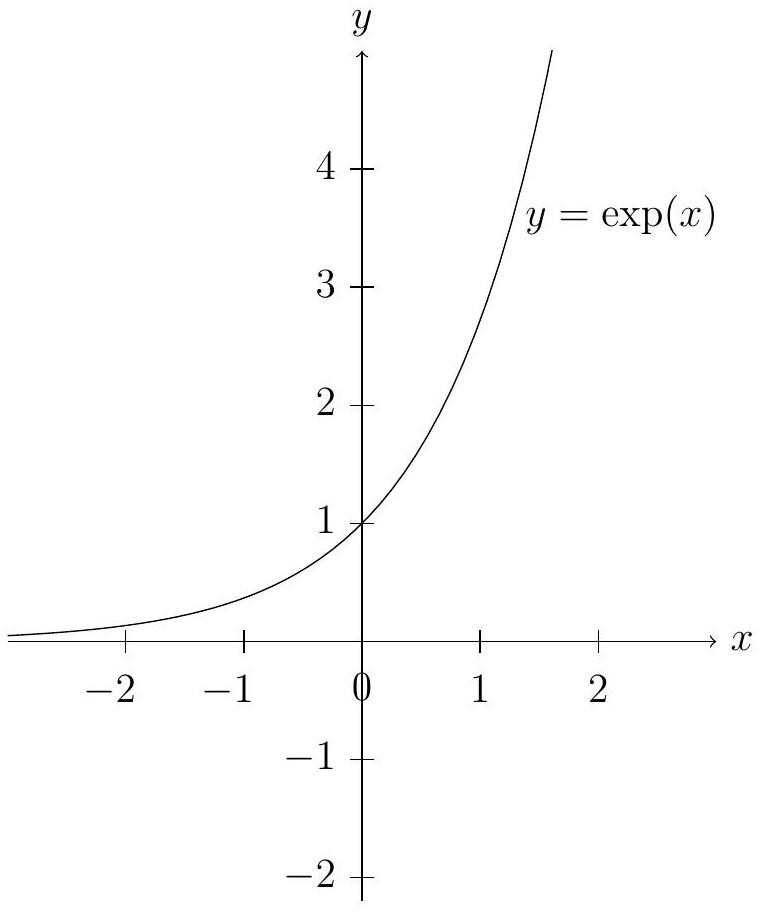
\includegraphics[width=0.4\textwidth]{2025_04_24_32a9930f7794b89a56a2g-5}
\end{center}

\begin{proposition}{}{}
  Pour tout $x \in \mathbb{R}, \quad \exp (x)>\hideM{0}$.
\end{proposition}

\begin{demo}
  Pour tout $x \in \mathbb{R}$,

  $$
  \exp (x)=e^{x}=e^{\frac{x}{2}+\frac{x}{2}}=e^{\frac{x}{2}} \times e^{\frac{x}{2}}=\left(e^{\frac{x}{2}}\right)^{2}
  $$

  Le carré d'un nombre réel est toujours positif donc $\exp (x) \geqslant 0$ et comme on sait que $\exp (x) \neq 0$, on en déduit le résultat.
\end{demo}

\begin{proposition}{}{}
  La fonction exponentielle est \hide{strictement croissante} sur $\mathbb{R}$.
\end{proposition}

\begin{demo}
  Par définition, $\exp$ est dérivable et pour tout $x \in \mathbb{R},(\exp (x))^{\prime}=\exp (x)$. Comme $\exp (x)>0$, on en déduit que exp est strictement croissante.
\end{demo}

\begin{method}{Étudier les variations d'une exponentielle}{}
  On dérive la fonction et on étudie le signe de la dérivée.\\
  Pour cela, on peut utiliser deux propriétés :

  \begin{itemize}
    \item Si $f$ est dérivable sur $\mathbb{R}$ alors $g: x \longmapsto f(a x+b)$\\
      est dérivable et pour tout $x, g^{\prime}(x)=a \times f^{\prime}(a x+b)$.
    \item Pour tout $x \in \mathbb{R}, \quad \exp (x)>0$.
  \end{itemize}
\end{method}

\begin{example}
  Etudier les variations de $g$ définie sur $\mathbb{R}$ par $g(x)=\exp (-3 x+7)$.

  ~\\Solution :\\
  $g$ est dérivable sur $\mathbb{R}$ comme composée de fonctions dérivables.\\
  Pour tout $x \in \mathbb{R}, g^{\prime}(x)=-3 \exp (-3 x+7)$.\\
  Or, pour tout $x \in \mathbb{R}, \exp (-3 x+7)>0$ donc $g^{\prime}(x)<0$.\\
  Ainsi, $g$ est strictement décroissante sur $\mathbb{R}$.
\end{example}

\begin{proposition}{}{}
  Pour tous $a, b \in \mathbb{R}$ :

  \begin{itemize}
    \item $a \leqslant b \Longleftrightarrow \hideM{\exp (a) \leqslant \exp (b)}$
    \item $a \geqslant b \Longleftrightarrow \hideM{\exp (a) \geqslant \exp (b)}$
    \item $a=b \Longleftrightarrow \hideM{\exp (a)=\exp (b)}$
  \end{itemize}
\end{proposition}

\begin{demo}
  \begin{itemize}
    \item Si $a \leqslant b$ alors, comme la fonction exponentielle est croissante, $\exp (a) \leqslant \exp (b)$. Réciproquement, supposons que $\exp (a) \leqslant \exp (b)$. On souhaite montrer que $a \leqslant b$. Supposons par l'absurde que $a>b$. Comme exp est strictement croissante, on aurait $\exp (a)>\exp (b)$, ce qui est une contradiction.
    \item Il suffit d'intervertir $a$ et $b$ dans la première proposition.
    \item D'après les deux premiers points, on peut écrire :
  \end{itemize}

  $$
  a=b \Longleftrightarrow a \leqslant b \text { et } a \geqslant b \Longleftrightarrow \exp (a) \leqslant \exp (b) \text { et } \exp (a) \geqslant \exp (b) \Longleftrightarrow \exp (a)=\exp (b) .
  $$
\end{demo}

\begin{remark}
  On peut démontrer ce genre de propriété pour n'importe quelle fonction strictement croissante. Attention néanmoins, la preuve de la réciproque a bien nécessité la stricte croissance de la fonction. En qénéral, si $f$ est croissante, on ne peut pas écrire que $f(a) \leqslant f(b) \Longrightarrow a \leqslant b$. Par exemple, si $f$ est une fonction constante sur $\mathbb{R}$, on a : $f(2) \leqslant f(1)$ et pourtant $2>1$.
\end{remark}

\begin{method}{Résoudre des équations ou des inéquations}{}
  \begin{itemize}
    \item On utilise les propriété algébriques afin de se rammener à des équations du type $e^{a}=e^{b}$ ou $e^{a} \leqslant e^{b}$.
    \item On applique ensuite la Proposition 10.
  \end{itemize}
\end{method}

\begin{example}
  Résoudre $e^{-2 x+1} \leqslant 1$

  ~\\Solution :\\
  Soit $x \in \mathbb{R}$ :

  $$
  \begin{aligned}
    e^{-2 x+1} \leqslant 1 & \Longleftrightarrow e^{-2 x+1} \leqslant e^{0} \\
    & \Longleftrightarrow-2 x+1 \leqslant 0 \\
    & \Longleftrightarrow x \geqslant \frac{1}{2}
  \end{aligned}
  $$
\end{example}

\begin{savoir}{}{}
\begin{itemize}
  \item Transformer une expression en utilisant les propriétés algébriques de la fonction exponentielle.
  \item Étudier le comportement de fonctions faisant intervenir la fonction exponentielle.
  \item Résoudre des équations et des inéquations faisant intervenir la fonction exponentielle.
  \item Modéliser une situation à l'aide de la fonction exponentielle.
\end{itemize}
\end{savoir}

\end{document}